\chapter{Project Governance}
\label{chap:projectGovernance}
\section{Roles and Responsibilities}
\label{sec:rolesResponsibilities}
\begin{tabularx}{0.95\linewidth}{%
  >{\raggedright\arraybackslash}p{0.1\linewidth}%
  >{\raggedright\arraybackslash}p{0.2\linewidth}%
  >{\raggedright\arraybackslash}X}
  \toprule
  Roles & Member & Responsibilities \\
  \midrule
  Business Owner
  & Jess and James
  & The business owners are the main Stakeholder of the team. They are responsible for determining the priority of upcoming work in the Backlog, get resources for the team, and modifying the Release Plan as necessary with the Product Owner.
  \\
  \midrule
  Product Owner
  & Yicun Tian, \newline Hongkang Li
  & The product owner is the spokesperson for the customer or stakeholders. Their primary responsibility is to ensure the product to-do list is transparent and clearly expressed, and everyone in the team has the same understanding of the project. Also, they are responsible for defining the product backlog with the Scrum master. They have no active role to play in daily stand-up, but they are welcome to attend.
  \\
  \midrule
  Scrum Master
  & Zhangfeng Qiu
  & The Scrum Master is the person in charge of the Scrum process. His primary responsibility is to guide the development team and communicate with product owners in daily development activities.
  \\
  \midrule
  Devlopment Team Members
  & Pin Wang, \newline Chongjing Zhang
  & The Scrum development team is composed of professionals who deliver the incremental work of "Done" products that may be released at the end of each Sprint.
  \\
  \midrule
  Subject Matter Expert
  & The teaching team -- mainly by Rajesh Chittor Sundaram.
  & The people with specialized knowledge or talent that is needed by the Team
  \\
  \bottomrule
  \\
  \caption{Roles and Responsibilitiest}  
  \label{tab:rolesResponsibilities}
\end{tabularx}

\clearpage
\section{Communication Plan}
\label{sec:communicationPlan}
Firstly, as a virtual team, we mainly use \textit{Slack} and \textit{Zoom} for information transfer, such as publishing message notifications, file sharing, etc. The link of each \textit{Zoom} meeting would be released by Scrum Master in the meeting channel of the project \textit{Slack} group. The Scrum Master is responsible for reminding the team to join the meeting in time. The meeting record would be provided by the Scrum Master. The example of our virtual meeting communication system is shown in Figure \ref{fig:meeting}.

\begin{figure}[htp]
\centering
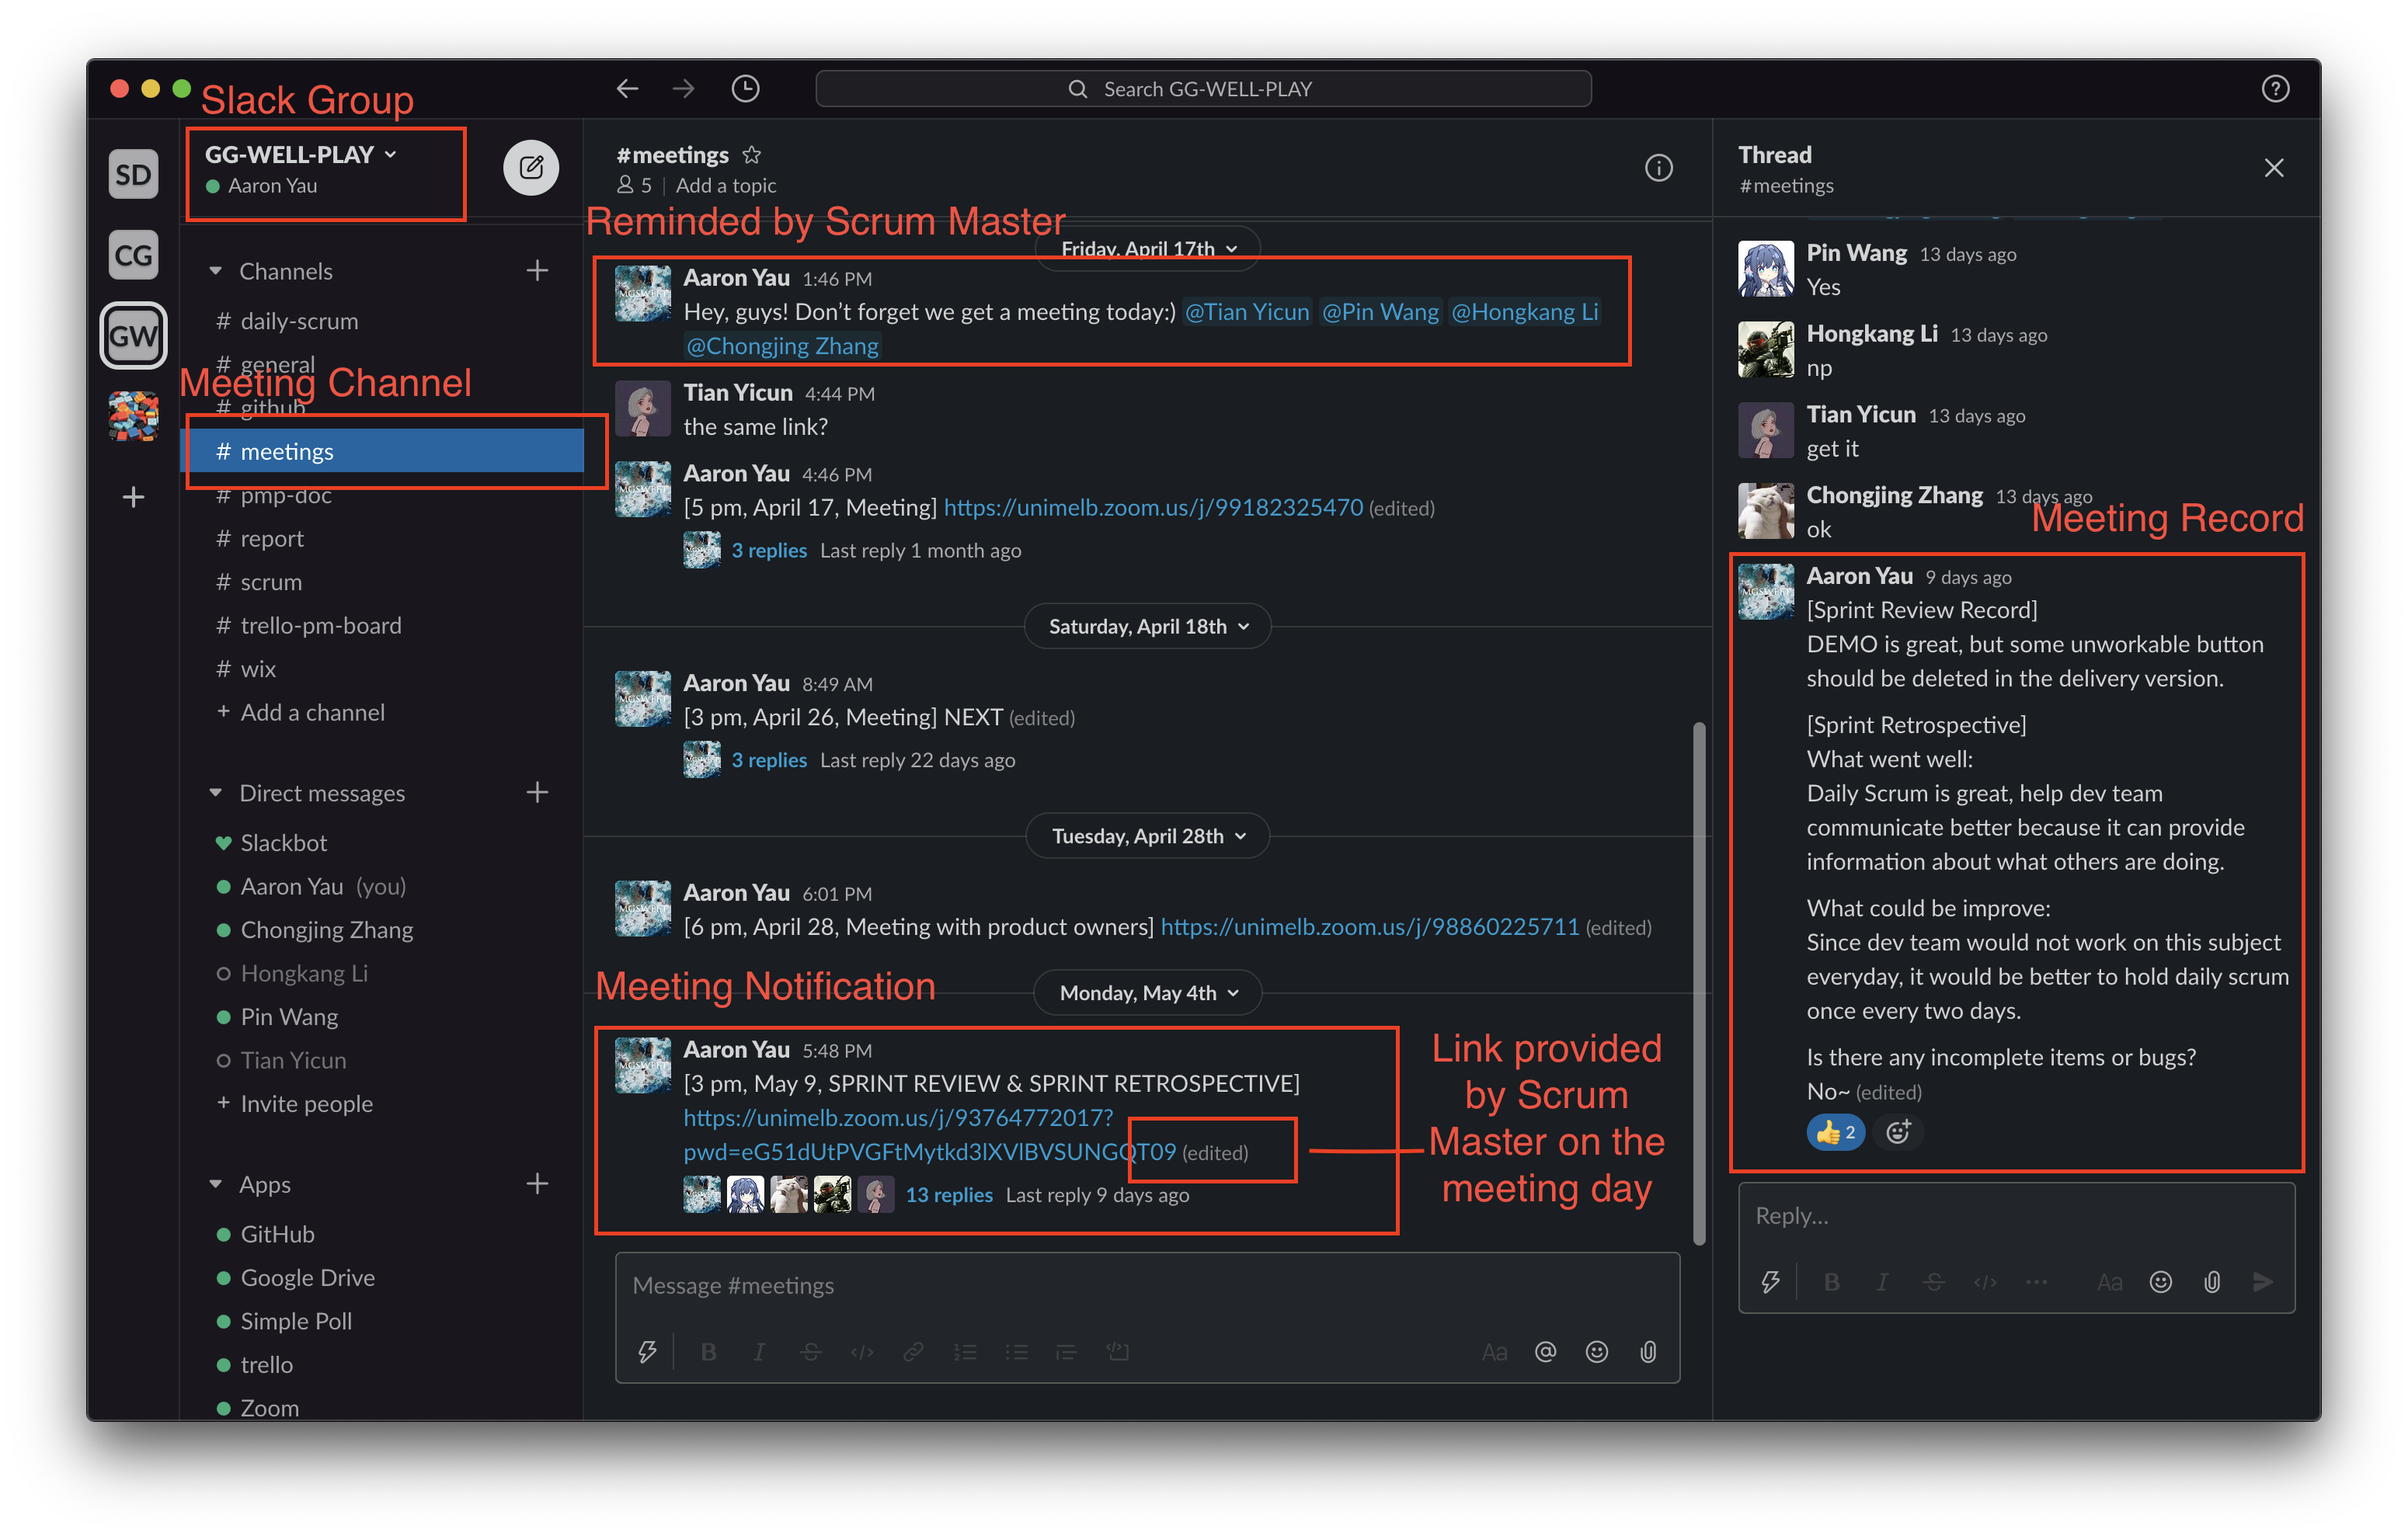
\includegraphics[width=\textwidth]{Figures/meeting.png}
\caption{Example of our Virtual Meeting Communication System}
\label{fig:meeting}
\end{figure}

Secondly, we use \textit{Trello} to help manage our Agile Board. Both the Project Backlog and the Sprint Backlog are managed on the Agile Board.

Furthermore, \textit{Github} is used to help enhance our teamwork and to manage our outcomes, such as the release of code and report.

According to the constraints of running a virtual team (Section \ref{sec:constraints}), we adjusted some of the communication processes in Scrum, and our communications matrix is shown in table \ref{tab:communicationMatrix}. 
\\

\begin{tabularx}{\linewidth}{%
  >{\raggedright\arraybackslash}p{1.5cm}%
  >{\raggedright\arraybackslash}p{2cm}%
  >{\raggedright\arraybackslash}X%
  >{\raggedright\arraybackslash}p{1.5cm}%
  >{\raggedright\arraybackslash}p{2cm}%
  >{\raggedright\arraybackslash}p{1.1cm}%
  >{\raggedright\arraybackslash}l}
  \toprule
  Processes & Stakeholder & Communication Objective & Format & Frequency & Owner & Importance
  \\
  \midrule
  Emergency Meeting
  & - Scrum Master
  \newline - Everyone in the team relative to the emergency meeting
  & To handle any unforseen emergency situation.
  & Virtual Meeting -- \textit{Zoom}; Formal Report
  & Anytime when needed
  & Scrum Master
  & High
  \\
  \midrule
  Project Planning Meeting
  & 
  - Scrum Master
  \newline - Product Owner
  \newline - Dev team
  \newline - Subject Matter Expert
  & Provide definition of the product backlog and provide a project plan for the whole project.
  & Virtual Meeting -- \textit{Zoom}; Formal Report
  & Weekly before the first sprint
  & Scrum master
  & High
  \\
  \midrule
  Sprint Planning Meeting
  & 
  - Scrum Master
  \newline - Product Owner
  & Provide Sprint Backlog, which selects high priority items from the Product Backlog that the Development Team can commit to delivering in a single Sprint.
  & Virtual Meeting -- \textit{Zoom}
  & At the beginning of each sprint:
  \newline - April, 27, 2020
  \newline - May, 11. 2020
  \newline - May, 25. 2020
  & Scrum master
  & High
  \\
  \midrule
  Daily Scrum
  & 
  - Scrum Master
  \newline - Product Owner
  \newline - Dev team
  & A short meeting used to start a day's work. Since we defined our features clearly, and every progress is shown in the Agile Board in \textit{trello}, we defined the importance of it to be medium.
  & Chat in the \textit{daily-scrum} channel of \textit{Slack}
  & Daily in the first sprint. In the second sprint, only held on:
  \newline - Monday
  \newline - Wednesday
  \newline - Friday
  & Scrum master
  & Medium
  \\
  \midrule
  Sprint Review
  & - Scrum Master
  \newline - Business Owner
  \newline - Product Owner
  \newline - Dev team
  & Show the demo of new features to Stakeholoders and get feedbacks from them.
  & Virtual Meeting -- \textit{Zoom}
  & At the end of each sprint:
  \newline - May, 8, 2020
  \newline - May, 22. 2020
  \newline - May, 30. 2020
  & Scrum master
  & Medium
  \\
  \midrule
  Sprint Retrospective
  & - Scrum Master
  - \newline - Business Owner
  - \newline - Product Owner
  - \newline - Dev team
  & An examination of what went well, what could be improved, etc. To make each Sprint more efficient and effective than the last.
  & Virtual Meeting -- \textit{Zoom}
  & At the end of each sprint
  \newline - May, 8, 2020
  \newline - May, 22. 2020
  \newline - May, 30. 2020
  & Scrum master
  & Medium
  \\
  \midrule
  Daily communication
  & - Anyone in the team
  & For exchanging information and better cooperation
  & Casual Chat on \textit{Slack} or personal \textit{Zoom} meeting.
  & Any working hours when needed
  & Anyone in the team
  & Low
  \\
  \bottomrule
  \\
  \caption{Communication Matrix}  
  \label{tab:communicationMatrix}
\end{tabularx}

\section{Risk Management}
\label{sec:riskManagement}
\subsection{Risk Impact Analysis Table}
\label{sec:riskImpactAnalysisTable}
We follow the following scoring rules to assess the impact of each risk:
\textit{(1) no impact; (2) minimal impact; (3) moderate impact; (4) severe impact; and (5) catastrophic impact;} The Risk Impact Analysis Table is shown in Table \ref{tab:riskImpactAnalysisTable}.

\begin{tabularx}{0.95\linewidth}{%
  >{\raggedright\arraybackslash}p{1cm}%
  >{\raggedright\arraybackslash}p{1.2cm}%
  >{\raggedright\arraybackslash}p{2cm}%
  ll%
  >{\raggedright\arraybackslash}X}
  \toprule
  Risk ID & Risk Type & Description & Probability & Impact & Justification\\
  \midrule
  1
  & Product
  & Design problem - The software developed by Wix has low scalability and is untransferable.
  & 60\%
  & 4
  & Although Wix can help quickly implement some basic functions, it may not be suitable for implementing the future enhancement of the project. There are many restrictions on creating a website on Wix. For example, the starter plan (\$5 per month) doesn't remove ads from the website, and there is no unlimited bandwidth or storage plan provided. You cannot build a high availability server in Wix. The site created by Wix is not transferrable.
  \\
  \midrule
  2
  & Business
  & Cancel orders maliciously or for no reason.
  & 3\%
  & 5
  & Malicious orders may cause unnecessary waste.  Some malicious buyers may intentionally create many orders and cancel them on the day of delivery. This kind of malicious actions may negatively affect the operation of the website and cause unnecessary loss. 
  \\
  \midrule
  3
  & Business
  & Email system or network system may fail.
  & 5\%
  & 2
  & If the email system or network system failed, the buyer would be unable to receive a confirming email after ordering. If clients were not able to receive feedback in time, they would not know whether their orders are confirmed or not. This situation may cause adverse effects on the user experience and cause unnecessary loss.
  \\
  \midrule
  4
  & Business
  & Service cancelation - Jess and James cannot deliver in time due to unforeseen circumstances.
  & 5\%
  & 1
  & Unforeseen circumstances like Jess and James getting sick or unnecessary travel ban may result in delivery cancelation. When they are unable to deliver, they have to provide reasons for their customer and cancel the order. Even though they may lose some money and customers may be disappointed, the impact of it would be small.
  \\
  \bottomrule
  \\
  \caption{Risk Impact Analysis Table}  
  \label{tab:riskImpactAnalysisTable}
\end{tabularx}

\subsection{Risk Register}
\begin{tabularx}{0.95\linewidth}{%
  >{\raggedright\arraybackslash}p{1cm}%
  >{\raggedright\arraybackslash}p{2cm}%
  >{\raggedright\arraybackslash}p{2cm}%
  >{\raggedright\arraybackslash}X%
  >{\raggedright\arraybackslash}p{2cm}%
  >{\raggedright\arraybackslash}p{2cm}}
  \toprule
  Risk ID & Trigger & Owner & Response & Response Strategy Type & Resources Required
  \\
  \midrule
  1
  & The new requirements proposed by Jess and James are confirmed by the development team that could not be implemented through Wix.
  & The development team
  & The development team can redevelop the whole system based on traditional web technics. Although it may take more time for the development team,  it can meet the needs of users. Also, keeping more reusable interfaces during development can help reduce the impact of this risk.
  & Mitigate or avoid 
  & The development team needs to keep more reusable interfaces during the development process.
  \\
  \midrule
  2
  & A user creates lots of orders in a short time and then cancels them without any reason. 
  & Jess and James
  & Limiting the number of times a user can cancel per week and limiting the time when the user cancels the order can help reduce the impact of this risk. For example, cancelation within 24 hours of the specified delivery time is not allowed. Also, customers would be asked to pay an advance deposit to reduce the economic loss caused by cancelation.
  & Mitigate
  & Jess and James need to spend effort to judge the reliability of the orders.
  \\
  \midrule
  3
  & Users complain that no confirmation email is sent to them.
  & Users(Jess \& James and customers)
  & If this risk occurs due to network failure, the system should be able to detect the user's network conditions and provide prompts automatically. The operation of the user to place an order is idempotent, which means that two identical operations will only operate once. If there is a problem with the function of auto-replying emails, the administrator of the maintenance system should be able to detect it in the background, the system is abnormal, and fix the bug in time.
  & Mitigate
  & The system needs to consume resources to detect the user's network environment and react to it.
  \\
  \midrule
  4
  & Jess or James is sick, or the government announced an unnecessary travel ban policy.
  & Jess and James
  & If an unnecessary travel ban policy is announced, Jess and James have to follow the rules and cancel their orders with an apology email sent to their customers. If the order cannot be delivered in time because the seller is sick or other assents, they can decide to hire another person to deliver or cancel their orders. It would be a trade-off between economic loss and user satisfaction loss.
  & Mitigate or accept
  & Hiring others for delivery would result in an economic loss, while cancelation of orders can bring negative effects to user experience.
  \\ 
  \bottomrule
  \\
  \caption{Risk Register}  
  \label{tab:riskRegister}
\end{tabularx}

\clearpage
\section{Technology}
\label{sec:technology}
The following are some technologies we researched for web development.
\begin{tabularx}{0.95\linewidth}{%l%
  >{\raggedright\arraybackslash}p{1.5cm}%
  >{\raggedright\arraybackslash}p{1.8cm}%
  >{\raggedright\arraybackslash}X%
  >{\raggedright\arraybackslash}X%
  >{\raggedright\arraybackslash}X}
  \toprule
  Name & Responsibility & Description & Pros & Cons \\
  \midrule
  Bootstrap
  & Front end framework
  & Bootstrap is a front-end framework that includes HTML and CSS based design templates and JavaScript plugins. It allows users to create responsive designs easily.
  & Easy to use and saves time; 
    Compatible with all browsers; 
    Responsive structures and styles;
  & Load time can be slow, file size can be huge; 
   All websites using Bootstrap look the same with out style customization;
  \\
  \midrule
  Foundation
  & Front end framework
  & Foundation is a front-end framework that is a collection of HTML, CSS and JS. It is a easy-to-use, powerful, and flexible framework for building web applications on any device.
  &  Fast development;  Adapt to all devices; Robust grid system;
  &  Community support is worse compare to Bootstrap; Need time to learn for beginners;
  \\
  \midrule
  Angular
  & Front end framework (JS)
  & Angular is a development platform for building web applications using TypeScript.
  & Component-based architecture allows reuse of components of UI, which is easy for writing tests; High performance; Fast development;
  & Difficult to manage components; Need time to learn for beginners; Lacks CLI documentation;
  \\
  \midrule
  React.js
  & Front end framework (JS)
  & React is a JavaScript library for building user interfaces. It can be used as the basis for developing web pages and mobile applications.
  & Components are modularized; Stable; Compatible with all browsers; Fast development;
  & Longer learning time than Angular; Lack of documentation; Less straightforward than pure JavaScript;
  \\
  \midrule
  Vue.js
  & Front end framework (JS)
  & Vue.js is an progressive, incrementally adoptable MVVM JavaScript framework for building user interfaces and single-page applications.
  & Clear documentation, simple to study; Small and fast; Components are modularized;
  & Too flexible that the codes are irregular; New framework, not very mature, has a smaller community;
  \\
  \midrule
  Java
  & Back end programming language
  & Java is a programming language that is class-based, object-oriented, and concurrent.
  & High-level language with simple syntax; Object-oriented programming allows reuse of codes; Supports multi-threading and distributed computing; Compatible for all platforms;
  & Slower than natively compiled languages; Less compact;
  \\
  \midrule
  PHP
  & Back end programming language
  & PHP is a server scripting language and a powerful tool for web development. It is fast, flexible and pragmatic that makes it easier to make dynamic and interactive web pages.
  & Compatible for all platforms; Easily embedded into HTML; High scalability; Large community;
  & Slower than other languages; Flexibility allows bad code;
  \\
  \midrule
  Python
  & Back end programming language
  & Python is an interpreted, high-level, general-purpose programming languages.
  & Easy to use and read; Multi-paradigm approach; Flexible;
  & Slower than natively compiled languages; Doesn't allow multi-threading;
  \\
  \midrule
  Django
  & Back end framework (Python)
  & Django is a Python-based high-level web framework follows MTV architectural pattern. It encourages rapid development and clean, pragmatic design.
  & Fast processing and developing; Scalable and flexible;
  & Not for smaller projects; Monolithic;
  \\
  \midrule
  Spring MVC
  & Back end framework (Java)
  & Spring MVC is a Java-based web framework that implements all the basic features of a core Spring framework like Inversion of Control and Dependency Injection.
  & Highly scalable and flexible; Use of modularity thus easy for testing; Large community;
  & Too complex, need time to learn for beginners; No clear guidelines;
  \\
  \midrule
  Express.js
  & Back end framework (Node.js)
  & Express is a minimal and flexible Node.js web application framework that provides a robust set of features for building web applications and APIs.
  & Fast development; Same language can be used to code front end; Simple; Flexible
  & Not for heavy projects;
  \\
  \midrule
  Wix
  & Web development platform
  & Wix is a popular cloud-based website builder. It provides an easy-to-use combination of powerful features that make it easy to build websites.
  & Flexible; Provides an app market; Easy to use; Massive template collection;
  & Loading is slow; Templates cannot be changed easily; Site cannot be transferred;
  \\
  \midrule
  Weebly
  & Web development platform
  & Weebly is a simple site builder with templates for great design. It allows the user to edit a website without any coding skills.
  & Massive template collection; Built-in support for e-commerce; Easy to use; Flexible;
  & Cannot add functionality not provided;
  \\
  \midrule
  WordPress
  & Web development platform
  & WordPress is a free and open source website builder. 
  & Powerful features; Scalability; Easy to use; Massive themes; A lot of free plugins;
  & Loading can be slow; Need to keep website updated; Doesn't support drag and drop;
  \\
  \bottomrule
  \\
  \caption{Available Web Development Technologies}  
  \label{tab:availableWebDevelopmentTechnologies}
\end{tabularx}
Among all technologies we researched above, we choose to use Wix content management system to build the website. Wix requires no coding skills or other usage of frameworks. It supports drag and drop to build web pages and provides a user-friendly UI to set the style of web components that integrates HTML and CSS from codes into user interfaces. And Wix also provides user-friendly UI to react to user actions with event handlers, this supports visualization of JavaScript. So far, Wix substitutes all front end languages or frameworks coding with user interfaces without any code. And Wix conceals the back end code in encapsulated apps, but also let users to implement customized logic using Node.js. Nonetheless, Wix offers a database operated by itself which also supports changes through graphical user interface. This database maintains the consistency of the usage of Wix platform, without extra database construction.

Compare to other website builders, Wix is more flexibly as it supports usage of Node.js to write customized backend code and take action when doing processes. And it already provides ready-made modules including online shop, user login, user permission management, and check out with credit card which can be used in developing the JJFresh website.

Take our project planning into consideration, we will need to implement all features of this website in 4 weeks. To complete the work on time, and not let it take too much time everyday as well, we want to be as efficient as possible, and also take use of the current existing web development tools to avoid building wheels. Nonetheless, we have the constraints that our development team members are not familiar with web development, no matter Wix or other frameworks and technologies.

By using Wix, we will save time of building and integrating the frameworks and adjusting the component properties with the help of visible user interface. And since we don't have much experience in web development, Wix's characteristic that it requires as least coding as possible is suitable us, and can help us focus on project management instead of catching up with the technology stacks. Therefore, we decided to use Wix to develop the website.

\section{Project Planning}
\label{sec:projectPlanning}
The SDLC of our project is Scrum. Since the key requirements for the initial development provided by Jess and James are fixed, a Fixed-Scope Release Planning would be used to plan our project.

\subsection{Product Backlog}
\label{sec:productBacklog}
The detail of product backlog is shown in Table \ref{tab:productBacklog}. \textit{Fabonacci sequence}\footnote{https://www.mountaingoatsoftware.com/blog/why-the-fibonacci-sequence-works-well-for-estimating} is used to provided relative estimation to both story point and value point.

The story points of different features are estimated by the development team and the Scrum master, based on the volume, risk, uncertainty and complexity of the features. We set the cost of the simplest feature (Edit admin account information) to 1 story point. And then estimate all other features' cost based on comparison with the simplest feature. 

The value points of the features are estimated by the product owners. We set the value of the least value feature (Edit admin account information) to 1 value point. And other features' values are estimated based on their relative value compared to the least value feature. 

BFTB Score is the abbreviate of the Bang-for-the-Buck\footnote{http://leftfoot.com.au/blog/struggling-with-relative-estimation-and-why-we-dont-use-time-watch-this} Score, which is a way of measuring how to get the most value in the shortest time. It is used to help assess the priority of the features. The BFTB Score is calculated by the formula below:
$$
  \text{BFTB Score} = \frac{\text{Value Point}}{\text{Store Point}}
$$

Initially, we define three milestones in our project. The first two milestones would be achieved at the end of the first sprint and at the end of the second sprint, respectively. Whether we would achieve the milestone depending on James and Jess's decision. Every milestone, we would release a runnable website to the market.
\begin{itemize}
\item The first milestone is to let the website go online without the function of purchase. The website can display all kinds of information about the products and provide the service of user registration. At the same time, the database is initially established to record the data of users and products.
\item The second milestone is to allow users to place orders to purchase products. After this milestone, sellers can view and modify user orders. Basic requirement testing has to be passed in this milestone.
\item The third milestone is to finish the future enhancement, which would not be considered in the initial development.
\end{itemize}

The features in Table \ref{tab:productBacklog} are ordered by their priority. The priorities are defined base on both the BFTB score and the development requirements. For example, even though the Database feature has a low BFTB score, because we can't record any data without it, its priority is still the highest.

Except for the three future user stories at the end of the product backlog table, all others are must-have stories because they are key requirements defined by Jess and James.
\begin{tabularx}{0.95\linewidth}{%
  l
  >{\raggedright\arraybackslash}p{3cm}%
  >{\raggedright\arraybackslash}X%
  p{1cm}p{1cm}p{1cm}
}
\toprule
Milestone & Feature & User Story & Story Point & Value Point & BFTB Score\\
\midrule
1
& Database
& As an admin, I need a database, so that I can store all the information of customers orders.
& 8
& 5
& 0.625
\\
\midrule
1
& Admin sign in and sign out
& As an admin, I want to provide my username and password, so that I can register an admin account.
& 2
& 2
& 1
\\
\midrule
1
& Manage product infomation
& As an admin, I want to manage product information, so that I can change the price or picture of my products.
& 5
& 3
& 0.6
\\
\midrule
1
& Browse product menu 
& As a customer, I want a menu that shows all the products, so that I can know what products are the website selling. 
& 8
& 5
& 0.625
\\
\midrule
1
& Customer sign up
& As customers, I want to sign up for the website, so that I can a member of the website.
& 2
& 2
& 1
\\
\midrule
1
& Customer sign in and sign out
& As customers, I should be able to sign in and sign out, so that I can manage my account and orders.
& 3
& 3
& 1
\\
\midrule
1
& Customer add and edit client information
& As customers, after login, I can add or edit my information like home address, user name, email address, and contact number.
& 2
& 3
& 1.5
\\
\midrule
2
& Add products to shopping cart
& As customers, after login, I can add or edit my information like home address, user name, email address, and contact number.
& 2
& 5
& 2.5
\\
\midrule
2
& Manage shopping cart
& As a customer, I want to manage my shopping cart, so that I can remove those I don't want or add some more products.
& 8
& 5
& 0.625
\\
\midrule
2
& Check out shopping cart
& As a customer, I want to choose the day and time for delivery, so that I can get the fruit on the right day.
& 8
& 5
& 0.625
\\
\midrule
2
& Cancel orders
& As a customer, I need to get the ability to cancel an order so that I can modify an order and then re-create.
& 2
& 2
& 1
\\
\midrule
2
& View and manage orders
& As an admin, I want the specific information of the user's order, so that I can packaging user orders.
& 8
& 5
& 0.625
\\
\midrule
2
& Register admin account
& As an admin, I need to get the ability to register for a new admin account, so that I can get more admin accounts if I need them.
& 1
& 1
& 1
\\
\midrule
2
& Edit admin account information
& As an admin, I may want to edit my admin account information, so that I can change the password.
& 1
& 1
& 1
\\
\midrule
3
& Add multiple bookings for the same slot
& As an admin, I want to add multiple bookings for the same slot in the future. So that I  can employ others to deliver boxes.
& 8
& 2
& 0.25
\\
\midrule
3
& Using AI to calculate delivery routes and times
& As an admin, I want to use AI technology to help me calculate an optimal route and time for delivery.
& 13
& 3
& 0.231
\\
\midrule
3
& Extended to allow for payment online.
& As an admin, I want to be paid online, so that I can save my time and improve the delivery efficiency.
& 13
& 3
& 0.231
\\
\bottomrule
\\
\caption{Product Backlog}  
\label{tab:productBacklog}
\end{tabularx}  

\subsection{Must-have Story Points}
Without calculating the features needed in the future, the total number of must-have story points is 60.
$$
SP_{total} = 60 \text{ (Story Point)}
$$

\subsection{Velocity Estimating (Re-estimate)}
There are two developers in our team. Since both of them are students, each of them can only spend about 1.2 to 3 hours a day on the project. They can work five days a week, so the total working hours of a week are 12 to 30 hours. We simply suppose each story point to be equivalent to one hour of working time. So the min velocity ($V_{min}$) for a two-week sprint is about 24 story points, and the max velocity ($V_{max}$) is about 60 story points. And by using the formula shown below, we can get our minimum and maximum number of sprints, which are 1 and 2.5, respectively. The velocity re-estimation burndown chart is shown in Figure \ref{fig:velocityEstimate}
$$
S_{min} = \frac{SP_{total}}{V_{max}}
\text{, } 
S_{max} = \frac{SP_{total}}{V_{min}}
$$
\begin{figure}[htp]
\centering
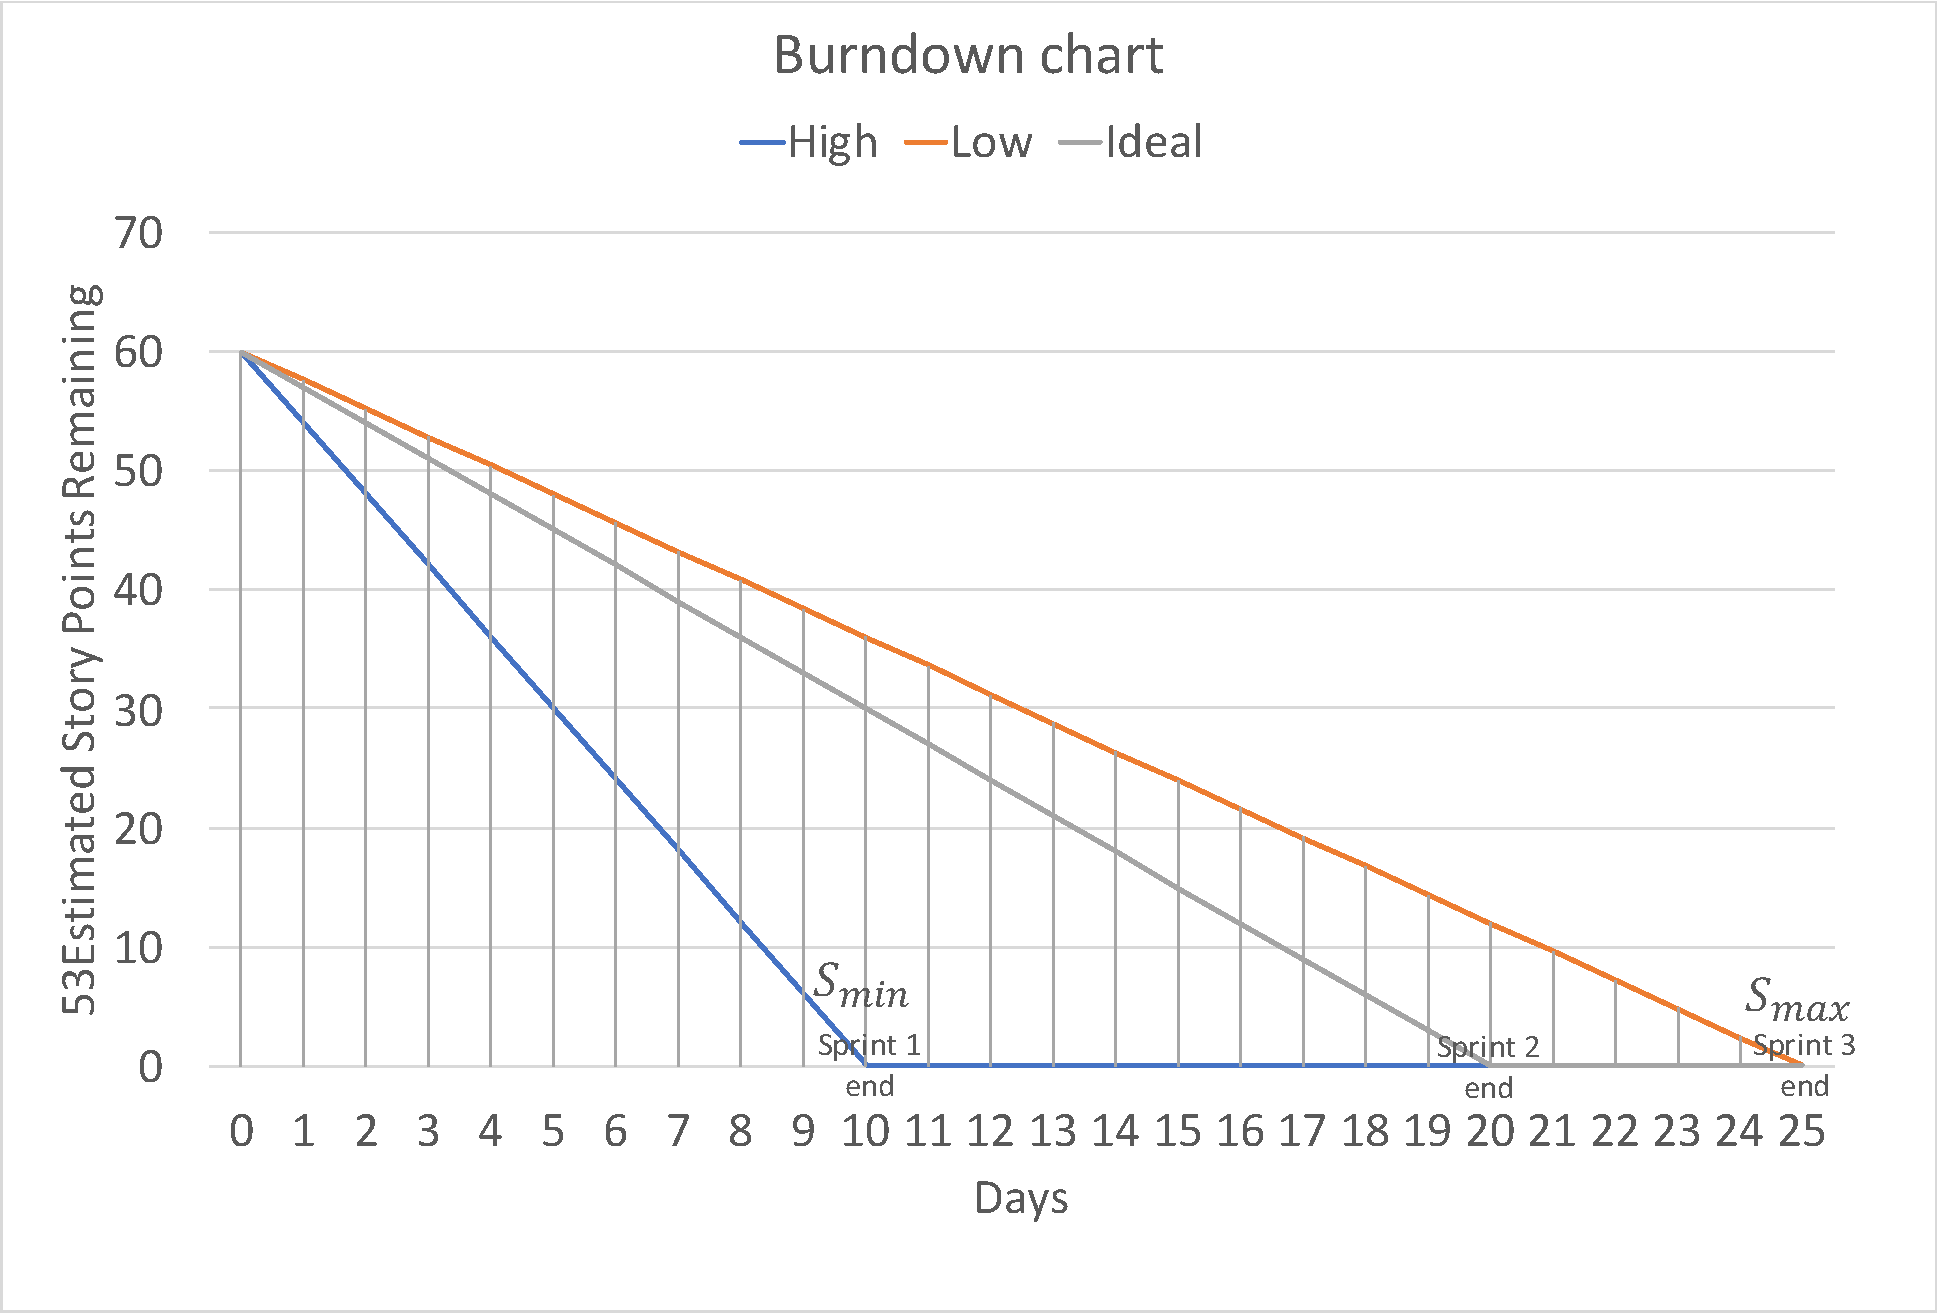
\includegraphics[width=0.9\textwidth]{Figures/velocityEstimate.pdf}
\caption{Velocity Re-estimation}
\label{fig:velocityEstimate}
\end{figure}

\clearpage
\subsection{Sprint Planning}
\subsubsection{Sprint Cycle}
\label{sec:sprintCycle}
The development phase of our project would start on \textbf{Monday, April 25}. Since the final delivery due date of the whole project is \textbf{June 1}, we decided to divide our development into three phases, each corresponding to a sprint.

The first phase is to let the website go online without the function of purchase. The website can display all kinds of information about the products and provide the service of user registration. At the same time, the database is initially established to record the data of users and products. The first sprint will last for two weeks, \textbf{from Monday, April 27 to Friday, May 8}. 

In the second phase, we need to realize the function that users place orders to purchase products, and sellers can view and modify user orders. Preliminary testing will also take place at this phase. The second sprint will last for two weeks, \textbf{from Monday, May 11 to Friday, May 22}.

The third stage is mainly based on user feedback to repair the vulnerability, carry out more tests and improve the existing functions. If some functions left over from the first two sprints are not implemented, they will also be solved in this sprint. As the project is nearing its end and there is less work left, the sprint in this phase will last only one week, \textbf{from Monday, May 25 to Friday, May 29.}

On \textbf{the first Monday of every sprint}, a Sprint Planning meeting would be held to select high priority items from the product backlog that the development team can commit to delivering in a single Sprint. The select itmes would be add to Sprint Backlog.

On \textbf{the last Friday of each sprint}, a Sprint Review meeting would be held to demonstrate the new features to Stakeholders, and a Sprint Retrospective meeting would be held to review the sprint.

A 15-minute Daily Scrum would be held \textbf{everyday} in the first sprint to start up the jobs. Everyone has to share what he/she did yesterday, what he/she plan to do, and what obstacles are slowing him/her.

\subsection{The First Sprint Plan}
As mention in Section \ref{sec:sprintCycle}, the main goal of the first sprint is to launch a webpage where customers can browse products. Considering both the BFTB Score, which is shown in Table \ref{tab:productBacklog} and the actual development needs, the Sprint Backlog of the first sprint is shown in table \ref{tab:firstSprintBacklog}. The total velocity and the delivery value of the first sprint is 30 story points and 25 value points, respectively. 
\\
\begin{tabularx}{0.95\linewidth}{%
  l%
  >{\raggedright\arraybackslash}p{2cm}%
  >{\raggedright\arraybackslash}X%
  >{\raggedright\arraybackslash}p{1cm}}
  \toprule
  Index & Feature & Tasks & Story Point\\
  \midrule
  1 
  & Database 
  & 1.Define the order model\textit{(1-hour)}; 2.Define the user information model\textit{(1-hour)}; 3.Define the admin information model\textit{(1-hour)}; 4.Create table and relation\textit{(2-hour)}; 5.Test\textit{(1-hour)}
  & 8
  \\
  \midrule
  2 
  & Browse product menu
  & 1.Provide a page for showing the list of the products\textit{(3-hour)}; 2.Show the types of the products\textit{(1-hour)}; 3.Show the price of the products\textit{(1-hour)}; 4.The price would change automatically\textit{(1-hour)}; 5.Show the pictures of products\textit{(1-hour)}.
  & 8
  \\
  \midrule
  3
  & Customer sign up
  & 1.Check whether the information of the user is valid\textit{(1-hour)}; 2.Add the user to the database and send a confirming email to the new member if valid\textit{(1-hour)}.
  & 2
  \\
  \midrule
  4
  & Customer sign in and sign out
  & 1.Sign in, check whether the user exist and whether the user's password correct\textit{(1-hour)}; 2.Sign out\textit{(1-hour)}; 3.Handle the problem of forgetting the user password (Allow password reset)\textit{(1-hour)}.
  & 3
  \\
  \midrule
  5
  & Customer add and edit client information
  & 1.Add and edit the name, email address, home address\textit{(1-hour)}; 2.Add and edit up to three multiple contact phone numbers\textit{(1-hour)}.
  & 2
  \\
  \midrule
  6
  & Manage product infomation
  & 1.Change the price of products\textit{(1-hour)}; 2.Change the pictures of products\textit{(1-hour)}; 3.Change the type of products\textit{(1-hour)}; 4.Add products\textit{(1-hour)}; 5.Delete products\textit{(1-hour)}.
  & 5
  \\
  \midrule
  7
  & Admin sign in and sign out
  & 1.Sign in\textit{(1-hour)}; 2. Sign out\textit{(1-hour)}.
  & 2
  \\
  \bottomrule
  \\
  \caption{The first Sprint Backlog (4.27 - 5.8)}  
  \label{tab:firstSprintBacklog}
\end{tabularx}

\subsection{The Second Sprint Plan}
\label{theSecondSprintPlan}
As mention in Section \ref{sec:sprintCycle}, the main goal of the second sprint is to allow users to place orders to purchase products. After this sprint, sellers can view and modify user orders. Basic requirement testing has to be passed in this sprint.

Following the feature development priority provided in Table \ref{tab:productBacklog}, the Sprint Backlog of the second sprint is shown in Table \ref{tab:secondSprintBacklog}. The total velocity and the delivery value of the first sprint is 30 story points and 24 value points, respectively. 

\begin{tabularx}{0.95\linewidth}{%
  l%
  >{\raggedright\arraybackslash}p{2cm}%
  >{\raggedright\arraybackslash}X%
  >{\raggedright\arraybackslash}p{1cm}}
  \toprule
  Index & Feature & Tasks & Story Pointt\\
  \midrule
  1
  & Add products to shopping cart
  & 1.Select size, type and amount of the products and add them to shopping cart.\textit{(2-hour)}
  & 2
  \\
  \midrule
  2
  & Manage shopping cart
  & 1.Select the items to pay\textit{(1-hour)}; 2.Change the amount of items\textit{(1-hour)}; 3.Delete items\textit{(1-hour)}; 4.View the price of the items selected\textit{(1-hour)}; 5.Provide a page to show all the items in the shopping cart\textit{(3-hour)}.
  & 8
  \\
  \midrule
  3
  & Check out shopping cart
  & 1.Choose a day and time for delivery.\textit{(1-hour)}. Only two bookings are allowed in a particular-hour.); 2.Send a confirming email to the customer\textit{(1-hour)}; 3.Show the day and time which is valid\textit{(2-hour)}; 4.Add an order to the user's order list\textit{(1-hour)}; 5.Handle synchronization problem\textit{(2-hour)}.
  & 8
  \\
  \midrule
  4
  & Cancel orders
  & 1.Cancel order\textit{(1-hour)}; 2.Send emails to both customer and admin\textit{(1-hour)}.
  & 2
  \\
  \midrule
  5
  & View and manage orders
  & 1.Confirm order\textit{(1-hour)}; 2.Order rank by date\textit{(1-hour)}; 3.Cancel order and provide reason\textit{(1-hour)}; 4.Provide a page to show order list with order information attach to it\textit{(4-hour)};
  & 8
  \\
  \midrule
  6
  & Register admin account
  & 1.Provide way for admin account registration\textit{(1-hour)}.
  & 1
  \\
  \midrule
  7
  & Edit admin account information
  & 1.Provide way for admin account information editing\textit{(1-hour)}.
  & 1
  \\
  \bottomrule
  \\
  \caption{The Second Sprint Backlog (May 11 - May 25)}  
  \label{tab:secondSprintBacklog}
\end{tabularx} 